%%
%%   sample.tex
%%

%% typeset: latexmk (uplatex -> dvipdfmx)
\documentclass[uplatex,dvipdfmx]{vkaishi}

\usepackage{vuccaken}
% \usepackage{v-hyperref}

\usepackage{sample}


\begin{document} % - - - - - - - 以下本文 - - - - - - - - - -

\mokuji{2} % 目次出力

%% - - - - - - - - - - - - - - - - - - - - - - - - %%
\kaishititle%
  {さんぷる}% title
  {テンプレ科学科4回生}% 所属
  {\vname{テンプレ}{太郎}}% name
%% - - - - - - - - - - - - - - - - - - - - - - - - %%

\helloLaTeX

%
\section*{はじめに}
会誌ではjsbookクラスを使用していますが,\texttt{vuccaken.sty}で少し上書きしています.\par
テーマが複数ある場合は別ファイルで作成してください.

%
\section{セクション}
このファイルのソースを自分のtexファイルにコピペしてお使いください.

%
\section{Cheat Sheet}

\subsection{数式環境}
(\ref{eq:complex})は最強の数式です.
\begin{align}
  z &= r e^{i\theta} \notag \\
    &= r (\cos\theta + i\sin\theta) \label{eq:complex}
\end{align}

\subsection{figure環境}
図\ref{fig:sin}はイケメンです.
\begin{figure}[htbp]
  \centering
  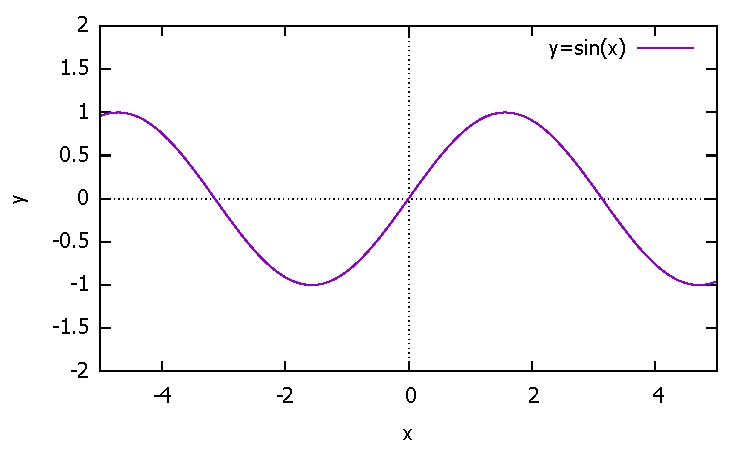
\includegraphics[width=0.5\textwidth]{img/fig-sin.pdf}
  \caption{$y=\sin x$のグラフ.gnuplotで作成した.}
  \label{fig:sin}
\end{figure}

\subsection{table環境}
表\ref{tbl:vegetable}は僕の主観です.
\begin{table}[htbp]
  \centering
  \caption{やさいの表}
  \label{tbl:vegetable}
  \begin{tabular}{r|ccc} \hline
    No. & やさい & いろ & 印象 \\ \hline
    1 & トマト & あかいろ & くさい \\
    2 & キャベツ & みどり & 無味乾燥 \\
    3 & かぼちゃ & きいろ & かたい \\
    4 & にんじん & おれんじ & ゴミ \\ \hline
  \end{tabular}
\end{table}

%% 参考文献
\begin{thebibliography}{99}
  \item 著者1・著者2,『本のタイトル』,出版社,出版年.
  \item ページの著者,『ページのタイトル』,最終アクセス日,\\
    (\url{https://vuccaken.github.io}).
  % \bibitem{キー1} 著者,『本のタイトル』,出版社,出版年.
\end{thebibliography}

\end{document} % - - - - - - - - - - - - - - - - - - - - -
%%
%% ファイトだよ!
%%